\documentclass[xcolor=dvipsnames]{beamer}
\usepackage{amsmath, amsfonts, epsfig, xspace, relsize}
\usepackage{algorithm,algorithmic, graphicx}
\usepackage{pstricks,pst-node}
\usepackage{multimedia}
\usepackage[normal,tight,center]{subfigure}
\setlength{\subfigcapskip}{-.5em}
\usepackage{beamerthemesplit}
\usepackage{mathtools}
\usepackage{xcolor}
\usepackage{fancyvrb}
\usepackage{framed,color}
\definecolor{shadecolor}{rgb}{0.8,1,0.5}
\usepackage{booktabs}
\renewcommand{\tablename}{表}
\renewcommand{\figurename}{圖}
\usepackage{IEEEtrantools}
\newcommand{\non}{\nonumber}
\setbeamertemplate{caption}[numbered]
\usepackage{multirow}
\usepackage{IEEEtrantools}
\newcommand{\non}{\nonumber}
\setbeamertemplate{caption}[numbered]
\usepackage{fontspec}  %加這個就可以設定字體
\usepackage{xecjk}       %讓中英文字體分開設置
%\setromanfont{LiHei Pro} % 儷黑Pro
\setmainfont{Times New Roman}
\newCJKfontfamily{\K}{標楷體}
\newCJKfontfamily{\H}{微軟正黑體}
\setmonofont[Scale=1]{Courier New} % 等寬字型
\setCJKmainfont[BoldFont=微軟正黑體]{王漢宗細圓體繁} %設定中文為系統上的字型,而英文不去更動,使用原TeX字型
\XeTeXlinebreaklocale "zh"             %這兩行一定要加,中文才能自動換行
\XeTeXlinebreakskip = 0pt plus 1pt     %這兩行一定要加,中文才能自動換行
%\usetheme{lankton-keynote}
\usetheme{Madrid}
\usecolortheme[named=BrickRed]{structure}
\author[蔡佳泓]{\K 蔡佳泓}

%\title[Statistical Methods for Social Sciences\hspace{.1em}\insertframenumber/\inserttotalframenumber]{Probability Theory}

\title[Statistical Methods for Social Sciences]{Regression Analysis\\
\smallskip
{\small {Introduction}}}

\date[5/16/2017]{2017年5月16日} %leave out for today's date to be insterted

\institute[ESC \& GIEAS]{\textbf{國立政治大學選舉研究中心暨東亞所}}

\begin{document}

\maketitle
\tableofcontents
\section{迴歸簡介}
\subsection{什麼是迴歸?}
\begin{frame} \frametitle{\K 迴歸的意義}
  \begin{itemize}
  \item 迴歸的目的是找到依變數或是反應變數(outcome)Y與一個或是一個以上的預測變數(predictor)X的函數關係。
  \item 迴歸的基礎觀念是條件機率,也就是迴歸線逼近在X成立的條件下,Y的平均值。所以模型的對象是$E[Y|X]$,也就是X變化時,Y的{\textcolor{red}{平均值}}變化大小。
 \item 母體迴歸函數(Population regression function)一般表示為$E(Y|X)=\beta_{0}+X\beta_{1}$。就是盡可能逼近X各類別下Y的平均數的函數。一旦找到這樣的迴歸函數,可以用來預測其他的觀察值,或是進行因果推論。
\end{itemize}
\end{frame}
\subsection{參數(Estimands), 樣本統計(Estimator), 估計(Estimates)}
\begin{frame}\frametitle{\H 迴歸分析的參數與估計}
\begin{itemize}
\item 參數:$E[Y|X]$是觀察不到的母體參數,所以模型的對象$E(Y|X)$。是因為我們只有一組樣本,所以得到的只是$E[Y|X]$的估計其中之一。
\item 樣本統計:$\hat{E}[Y|X]$。
\item 估計:某一個樣本所得到的$\hat{E}(Y|X)$。
\end{itemize}
\end{frame}

\section{Non-parametric regression}
\subsection{無母數迴歸}
\begin{frame}\frametitle{\H 無母數迴歸的意義}
\begin{itemize}
\item 母數模式意為函數是由一組母數所規範;具有某種固定的型態,例如線性、對數等等。無母數的模式則為未知的函數型態,簡單地講,也就是沒有母數的限制。
\item 母數迴歸模式的最大優點是可以推論迴歸結果,但是其缺點就是迴歸形式固定而呆板。無母數迴歸的優點是符合資料程度高,但是難以推論。
\item 無母數迴歸不假設變數之間有線性關係,目的是選擇合適的平滑參數,讓通過樣本的迴歸線能夠最好地逼近真實的迴歸曲線,也就是讓均方誤差為最小。
\end{itemize}
\end{frame}
\begin{frame}\frametitle{\H 無母數迴歸的重要性}
\begin{itemize}
\item 無母數迴歸可以作為測試最小平方法迴歸模型是否線性的基礎。
\item 無母數迴歸及散佈圖可以作為瞭解資料分佈的基礎,有可能是非線性分佈。
\item 無母數迴歸係數無法像線性迴歸係數,可以進行$t$檢定或是推論母體的參數。它只能讓我們觀察最接近每一個點的線。
\end{itemize}
\end{frame}
\subsection{區域平均值(Simple Local Average)}
\begin{frame}\frametitle{\H 區域平均值}
\begin{itemize}
\item 估計$E[Y|X]$的方法之一是「可移動的區域平均」(moving local average)。假設$[X_{0}-h,X_{0}+h]$這個區間內有許多y,計算這些y的平均值便是「可移動的區域平均」。
\item $h$稱為帶寬(bandwidth)。
\item 如果在區間內的每一個y都視為同樣的,有相同的權重,稱為「單一核密度」(Uniform Kernel)。又稱為Nadaraya–Watson kernel regression estimate.
\item 母體參數可估計如下:
\begin{center}
$\hat{E}[Y|X]=\frac{\sum_{i=1}^N K_{h}((X_{i}-x_{0})/h)Y_{i}}{\sum_{i=1}^N K_{h}((X_{i}-x_{0})/h)}$
\end{center}
\end{itemize}
\end{frame}
\begin{frame}\frametitle{\H 區域平均值}
\begin{itemize}
\item 根據以上「可移動的區域平均」公式,依照不同的帶寬,可計算得到不同的區域平均值。
\item 將這些區域平均值連起來就是無母數迴歸線。

\end{itemize}
\end{frame}
\begin{frame}\frametitle{\H 無母數迴歸圖1: Kernel}
\begin{figure}
\begin{center}
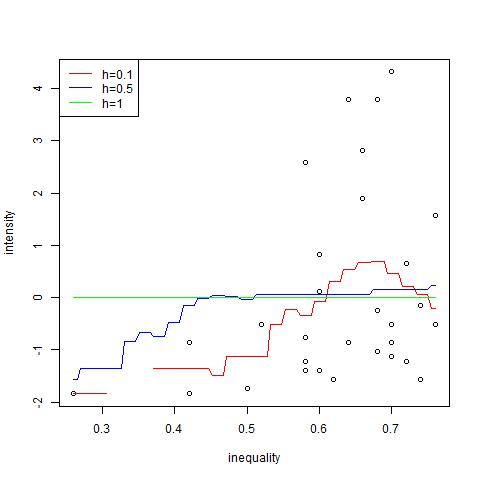
\includegraphics[scale=.45]{nonpreg1.jpg}
\end{center}
\end{figure}
\end{frame}
\subsection{Local weighted polynomial regression}
\begin{frame}\frametitle{\H 區域多項迴歸}
\begin{itemize}
\item 前一個無母數迴歸中,因為每一區間內的觀察值得到同樣的權重,所以形成線條狀的迴歸線。
\item 在資料中我們取若干觀察值來計算每一個觀察值到特定觀察值(focal point)之間的距離,不同的區間大小決定該區間會用到多少比例的觀察值,也決定曲線的平滑程度。區間越大,平滑程度越大。。
\item 進一步,我們用多元的函數來決定權重。根據權重可以計算出特定觀察值的模型值。模型可表示為:
\begin{center}
$Y_{i}=\alpha_{0}+\beta_{1}(x_{i}-x_{0})+\cdots +\beta_{p}(x_{i}-x_{0})^{p}+E_{i}$
\end{center}
\item 在最小化誤差的平方之後,把估計點連起來平滑曲線,稱為local weighted polynomial function或是Bivariate local polynomial regression. 
\item 這個只用鄰近資料點的方法,可以避免某些特別大或是特別小觀察值的影響。
\end{itemize}
\end{frame}
\begin{frame}\frametitle{\H 無母數迴歸圖2: LOESS}
\begin{figure}
\begin{center}
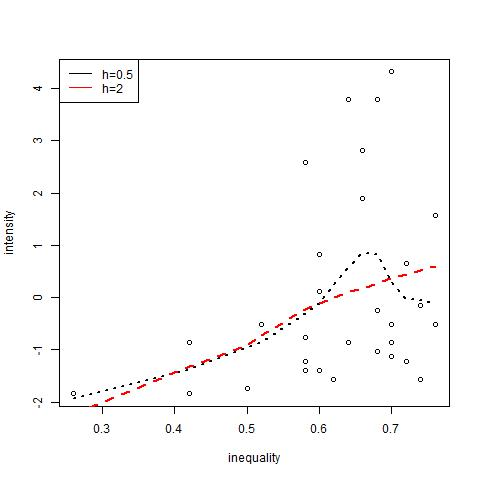
\includegraphics[scale=.4]{nonpreg2.jpg}
\end{center}
\end{figure}
\end{frame}
\begin{frame}\frametitle{\H 合併}
\begin{itemize}
\item 合併線性迴歸與無母數迴歸在一張圖,可以看出資料點的散佈並非線性。
\item 有許多診斷反應變數與解釋變數是否有線性關係的方式,例如檢視預測值與殘差的散佈圖,如果散佈圖呈現特定形狀,有可能兩者之間非線性關係。
\end{itemize}
\end{frame}
\begin{frame}\frametitle{\H 線性迴歸與無母數迴歸圖}
\begin{figure}
\begin{center}
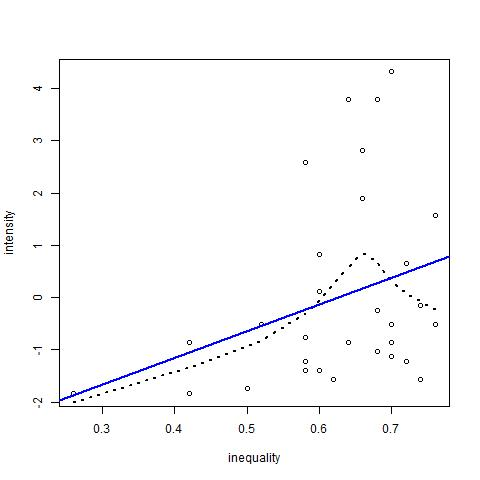
\includegraphics[scale=.45]{nonpreg3.jpg}
\end{center}
\end{figure}
\end{frame}
\begin{frame}\frametitle{\H 無母數迴歸}
\begin{itemize}
\item 從點估計的均方誤差和可以想像,變異數與誤差之間有衝突,一個太大,另一個就會太小。
$MSE_{pred.-y_{i}}=Var_{pred.}+Bias_{\mathit{f_{i}}-y_{i}}^2$
\medskip

\item 無母數迴歸使用的樣本統計(estimator)有很大的彈性。\item 帶寬越小,越有彈性,預測值的變異數也越大。
\item 帶寬越大,越不具彈性,與真實模型之間的誤差越大。
\end{itemize}
\end{frame}
\begin{frame}\frametitle{\H 4個區間}
\begin{center}
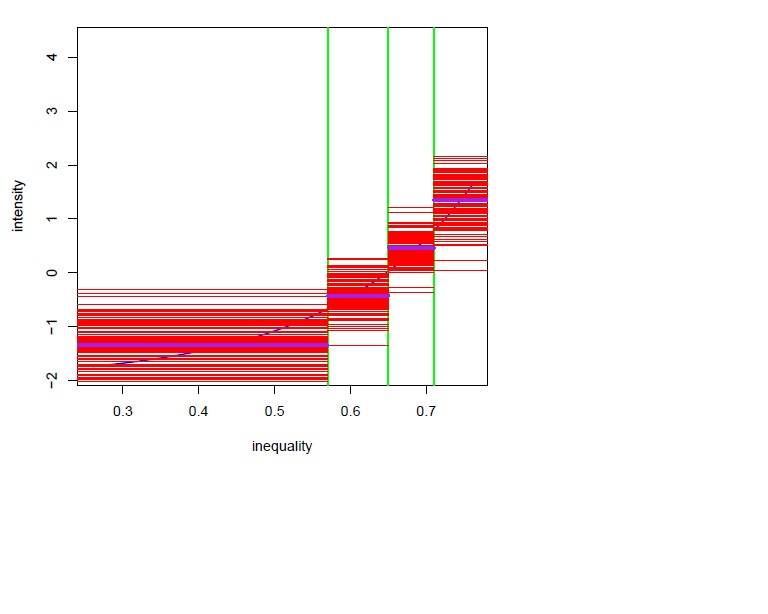
\includegraphics[scale=.64]{nonpa_4.jpg} 
\end{center}
\end{frame}
\begin{frame}\frametitle{\H 8個區間}
\begin{center}
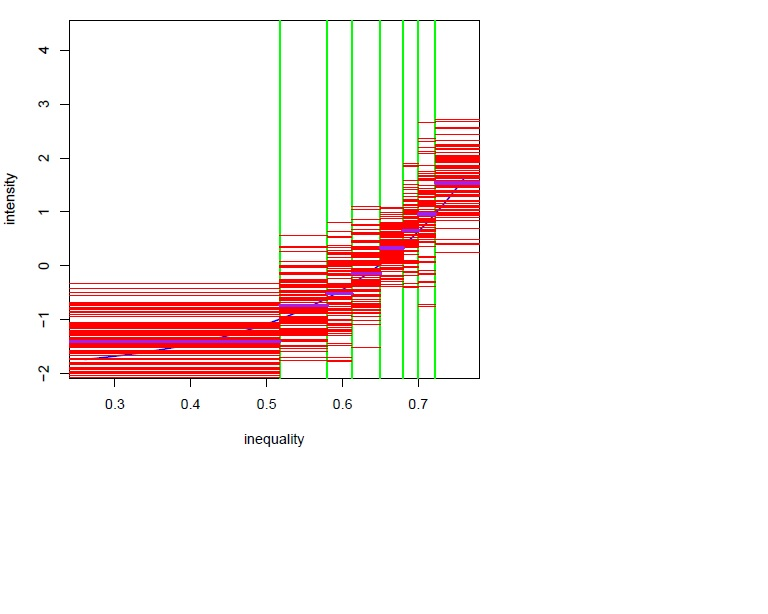
\includegraphics[scale=.65]{nonpa_8.jpg} 
\end{center}
\end{frame}
\begin{frame}\frametitle{\H 實例}
\begin{center}
\includegraphics[scale=.4]{scatter1.jpg} 
\end{center}
\end{frame}
\begin{frame}\frametitle{觀察值與線性迴歸預測值}
\begin{center}
\includegraphics[scale=.5]{fitline.jpg} 
\end{center}
\end{frame}
\begin{frame}\frametitle{\H 線性與無母數迴歸}
\begin{center}
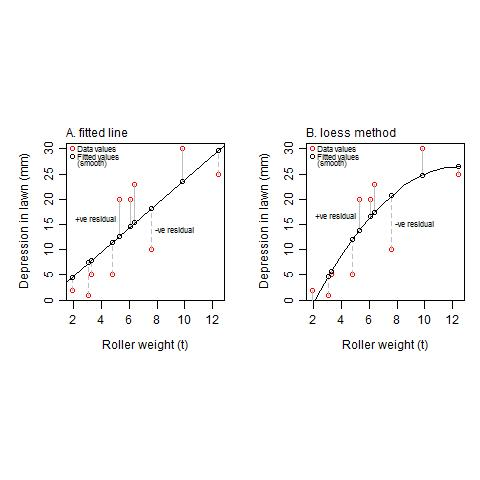
\includegraphics[scale=.6]{loess_r.jpg} 
\end{center}
\end{frame}
\begin{frame}[fragile=singleslide]{實際操作}
\begin{itemize}
\item \tt{R} 有 \tt{LOESS} 函數
\bigskip
\begin{Verbatim}[frame=single,label=R code,
fontseries=b,xleftmargin=2mm,commandchars=\\\{\},
formatcom=\color{blue}]
plot(Chirot$inequality,Chirot$intensity)
with(Chirot,lines(lowess(inequality, intensity, f=0.6, iter=0))
abline(lm(Chirot$intensity ~ Chirot$inequality))
\end{Verbatim}
\end{itemize}
\end{frame}
\section{有母數統計:線性迴歸}
\subsection{意義}
\begin{frame}\frametitle{\H 線性迴歸}
\begin{itemize}
\item 線性迴歸假設條件平均值呈現線性。
\begin{center}
$E[Y|X]=\beta_{0}+X\beta_{1}$
\end{center}
\item 只有兩個係數。$ \beta_{0} $稱為截距或常數,$ \beta_{1} $稱為斜率係數。
\item 線性假設的其中之一是截距為固定。
\item 也可表示為:
\begin{center}
$Y=\hat{\beta}_{0}+\hat{\beta}_{1} X  $\\
%intensity=-3.2+5.1 inequality
\end{center}
\item 例如:叛亂強度與社會不平等的線性關係估計為:
\begin{center}
intensity=-3.2+5.1 inequality
\end{center}
\end{itemize}
\end{frame}
\begin{frame}
\begin{figure}
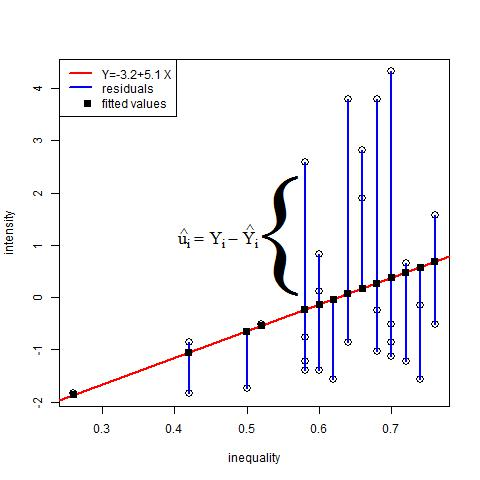
\includegraphics[scale=.45]{reg1.jpg} 
\caption{迴歸線圖}
\label{fig:fig1}
\end{figure}
\end{frame}
\subsection{線性迴歸的解釋}
\begin{frame}\frametitle{\H 線性迴歸的解釋:$\beta_{0}$}
\begin{center}
$Y=\hat{\beta}_{0}+\hat{\beta}_{1} X $\\
intensity=-3.2+5.1 inequality
\end{center}
\begin{itemize}
\item $\hat{\beta}_{0}$的意義為何?
\item 如果$X=0$,$E[Y|X=0]=  \hat{\beta}_{0}$ 。
\item 平均來說叛亂強度是-3.2,當該國的不平等指數為0。
\end{itemize}
\end{frame}
\begin{frame}\frametitle{\H 線性迴歸的解釋:$\beta_{1}$}
\begin{center}
$Y=\hat{\beta}_{0}+\hat{\beta}_{1}X   $\\
intensity=-3.2+5.1 inequality
\end{center}
\begin{itemize}
\item $\hat{\beta}_{1}$的意義為何?\\
方向:\\
$\beta_{1}>0$: $E[Y|X]$ 隨著X增加\\
$\beta_{1}<0$: $E[Y|X]$ 隨著X減少\\
$\beta_{1}=0$: $E[Y|X]$與X無線性關係
\end{itemize}
\end{frame}
\begin{frame}\frametitle{\H 線性迴歸的解釋:$\beta_{1}$}
\begin{center}
$Y=\hat{\beta}_{0}+\hat{\beta}_{1}X   $\\
intensity=-3.2+5.1 inequality
\end{center}
\begin{itemize}
\item $\hat{\beta}_{1}$的意義為何?\\
強度:\\
$\beta_{1}$告訴我們隨著X增加或是減少一個單位,平均而言Y會多快增加或是減少一個單位。\\
不平等每增加一個單位,叛亂強度平均會增加5.1個單位。
\end{itemize}
\end{frame}
\subsection{預測}
\begin{frame}\frametitle{\H 預測}
\begin{itemize}
\item 線性迴歸可以預測新的觀察值。
\item 步驟:
\begin{enumerate}
\item 估計樣本的$\hat{\beta}_{0}$以及$\hat{\beta}_{1}$。
\item 根據$\hat{E}[Y|X=x_{new}]=\hat{\beta}_{0}+\hat{\beta}_{1}x_{new}$得到新的預測值$\hat{E}[Y|X=x_{new}]$
\end{enumerate}
\item 同樣步驟,可估計不同觀察值下的依變數的差異:
\begin{center}
$\hat{E}[Y|X=x_{new,1}]=\hat{\beta}_{0}+\hat{\beta}_{1}(x_{new,1})$\\
$\hat{E}[Y|X=x_{new,2}]=\hat{\beta}_{0}+\hat{\beta}_{1}(x_{new,2})$\\
$\hat{E}[Y|X=x_{new,1}]-\hat{E}[Y|X=x_{new,2}]=\hat{\beta}_{1}(x_{new,1}-x_{new,2})$
\end{center}

\item $\beta_{1}$可以解釋為兩個差別一個單位的觀察值所造成的Y的變化。

\end{itemize}
\end{frame}
\subsection{因果推論}
\begin{frame}{\H 因果推論}
\begin{itemize}
\item $ \beta $ 可以用來描述以及預測。
\item 如果以下兩個條件成立,迴歸的結果可以推論因果關係:
\begin{enumerate}
\item $E[Y|X]$有線性關係。
\item 除了X之外沒有其他影響Y的變數,稱之為外生性(exogeneity)。
\end{enumerate}
\item 利用無母數迴歸或者是非線性迴歸,可以讓資料滿足條件一。
\item 加入適當的{\textcolor{red}{控制變數}},可以減少其他變數的影響,以滿足條件二。
\item 用研究設計避免解釋變數與其他變數混雜的情形。
\end{itemize}
\end{frame}

\begin{frame}\frametitle{\H 總結}
\begin{enumerate}
\item {\K 瞭解線性迴歸的前提}
\item {\K 瞭解何謂無母數迴歸}
\item {\K 瞭解線性迴歸的意義}
\item {\K 瞭解線性迴歸的預測以及因果推論}
\end{enumerate}
\end{frame}

\end{document}
